%!TEX root = prelim.tex
%!TEX root = fakeroot.tex

%\subsection{Optimizing the Speed of the Recognition Algorithm}



\frame{\frametitle{Parallelization of the Algorithm}
\begin{itemize}
\item Recognition on database of 100 training users with 30 training images per user takes about 5 minutes.
\item Needs to execute in about a second to be useful for access control.
\item To get this sort of speedup
\begin{itemize}
\item Coarse Grained Parallelism: Farm out Per-User alignment to multiple machines $\Rightarrow$ about 3x speedup.
\item Fine Grained Parallelism: Operations on entire images are amenable to GPU implementation $\Rightarrow$ about 100x speedup.
\end{itemize}
\end{itemize}
}
%
%\frame{\frametitle{Timing}
%\begin{table}[h]
%\begin{tabular}{|c|c|}
%\hline
%Operation & Execution Time (seconds)\\
%\hline
%Loading the training database & 74\\
%\hline
%Per-user alignment & 130\\
%\hline
%Resampling the training images & 18\\
%\hline
%Final recognition step &137\\
%\hline
%\end{tabular}\vspace{2mm}
%\caption{Execution timing for a database of 100 training users with 30 xga grayscale training images per user} \label{tab:breakdown}
%\end{table}
%}

%Enormous amount of data
%Problem is very data parallel





%%\subsection{Factors causing the current implementation to run slowly}
%%\label{sec:factors}

%Before any progress can be made on improving the speed of the algorithm, we must first understand why it currently runs so slowly. The main reason is that the sparsity based alignment and recognition algorithms detailed in the previous chapters use entire images as features.  Many face recognition algorithms either start with much smaller features to begin with (i.e. image patches, SIFT features), or project the images down to a much lower dimension as a first step.  Not only are we using relatively large training images in their natural basis, we are performing optimizations on them repeatedly in a loop, instead of just once, as is the case with Eigenfaces.   These optimization routines involve operations on many of these images at a time (for example, the recognition step currently uses 38 training images).  This is a very expensive algorithm in terms of the amount of data that must be handled simultaneously, and would have been considered very impractical to implement until rather recent improvements in computing hardware.  

%While we have an enormous amount of data that must be operated on, the simplicity of our choice of features has resulted in an algorithm that is extremely data parallel.  Table \ref{tab:breakdown} shows a breakdown of the execution time for the different parts of the algorithm.  The first thing to note is that the algorithm's execution time will have to be improved by a factor of about 100 in order to be useful for access control.  It is unreasonable to expect a user to wait for much more than a second while the system decided whether or not to unlock the door.  Due to the emergence of readily available massively parallel processors in the form of programmable GPU's, this factor of speed improvement is actually more reasonable than it sounds.  Similar speedups have actually been achieved for some other data parallel tasks when ported from the CPU to the CUDA architecture.  The next few subsections will outline some strategies for optimizing the individual steps.

%%{\bf Loading the training database}  
%\subsection{Loading the training database}  
%The training database can be potentially quite large; for a database of 100 users, the full resolution training images take up 3 GB of data.  While his can be reduced significantly for the per-user alignment step (we only need the smaller re-sampled training images), we will need to load the full resolution images for the users that make it to the final recognition step, and this access must happen with very low latency.  Clever management of the loading of training images into memory will clearly be necessary.

%One strategy for reducing the latency of the image loading is to use a technology called memory mapping.  This creates a mapping between the data in a file in the system (most of which will be resident on the hard drive) and the address space of the program.  The operating system's virtual memory system then handles the loading of data from disk into RAM as needed when the program access the corresponding addresses in its memory space.  This technique has the potential to kill several birds with one stone:
%\begin{itemize}
%\item Since there is one virtual memory system for all processes in the os, portions of the database that are used by multiple processes can share the data that has been loaded into RAM.  This can significantly reduce the memory footprint when multiple instances of the recognition system are running simultaneously.
%\item It is much easier to load just the portion of each image file that is needed.  Resampling the training images will only require a subset of the pixels from the high resolution image.  On x86 systems the memory page size is 2KB.  For a grayscale xga image laid out linearly one disk this corresponds to two rows of the image.  In this case only the rows that overlap the user's face will get loaded from disk into memory.  This can be improved further by laying out the data so that each memory corresponds to a tile of about 45 x 45 pixels.  Then only the tiles that overlap the users' face will have to get loaded into memory.
%\item There is a mechanism to hint to the operating system what data will be needed in advance so that is can be pre-loaded.  
%\end{itemize} 
%Another strategy for reducing the latency of the image loading is to try to predict which images will need to be loaded in advance of when they are used.  In particular, we have some information about which users will likely make the cut for the recognition step while per-user alignment is still being performed.  Any training user that is not in the top $S$ (currently set to 10) users aligned so far certainly need not be loaded into memory.  

%%{\bf Per-user alignment}  
%\subsection{Per-user alignment}  
%Since this operation must be performed once per training user, the cost of this operation grows proportionally with the size of the training database.  For each user, the computation for this step involves repeatedly solving an l1 optimization problem and resampling filtered versions of the test image.  

%One strategy for reducing the amount of time spent resampling(warping) the training images is to make use of the fact that we are resampling $N$ (= 38 training images currently) simultaneously with the same transformation.  We can use this fact in two ways: first, we only have to compute the mapping of the pixel locations once, and second, we can tile the data for all 38 images together to further reduce time spent accessing memory.   

%%{\bf Resampling the training images}  
%\subsection{Resampling the training images}  
%Again, clever tiling and pre-fetching will be able to greatly reduce the time spent in this task.

%%{\bf Final recognition step}  
%\subsection{Final recognition step}
%This bulk of the time spent in the final recognition step is in a large l1 optimization.  The matrices involved are bigger, but the l1 optimization problem only has to be solved once.  

%The two l1 optimization problems are solved by re-casting them as linear programming problems.  The resulting linear programming problems can be solved efficiently using interior point methods.  The most expensive operation in the interior point method for these problem sizes is the computation of the step direction.  This requires a multiplication of several large matrices to compute the matrices for a much smaller linear system of equations.  This smaller linear system is then solved by minimizing the $\ell^2$ norm of the error.  Since all of these operations are taking place on very large arrays, these optimizations have the potential to map well to massively programming architectures, such as GPU's.  The massively parallel (capable of executing hundreds of threads concurrently) architecture that is currently the most promising is Nvidia's CUDA architecture, and development will center on this development system for the foreseeable future.  Performance gains of up to 100x over CPU implementations have been reported for algorithms that map well to the GPU.

%An example of an operation in our algorithm that is very low hanging fruit for GPU implementation is the multiplication of $A^T * D * A$ where $A$ is extremely tall (5120 x 38) and $D$ is diagonal.  While a general GPU implementation of matrix multiplication is provided with the GPU, there are likely significant performance improvements to be gained from a custom multiplication routine.  Data can be shared between the left and right copies of A.  To conserve cache space $A$ can be stored as the original 8 bit data type that came from the image, along with a floating point scale factor for each column.  The fact that $D$ is diagonal also greatly reduces the amount of computation that need be done.  Since $A$ is extremely tall, the edge case (in computation and in memory loading) for  the long edge is much more important that for the short edge.  Furthermore, the prior knowledge that $D$ gets updated about 10 times as frequently as $A$ how best to handle memory transfers.

%While the efficient implementation of the sparse representation algorithms we used has a limited interest from a theoretical standpoint, it is absolutely critical for enabling the use of these techniques for vision applications.  Sparse representation may one day be as important a building block for computer vision as the singular value decomposition is currently, but this cannot happen without efficient implementations that are tuned both for the application domain and the available hardware.  



%\frame{
%\frametitle{Loading the training database}
%\begin{itemize}
%\item
%\item
%\item
%\end{itemize}
%}

%\subsection{Optimizing the Speed of the Recognition Algorithm}
%\frame{\tableofcontents[currentsection, currentsubsection]}

%\frame{
%\frametitle{Loading the training database}
%\begin{center}
%%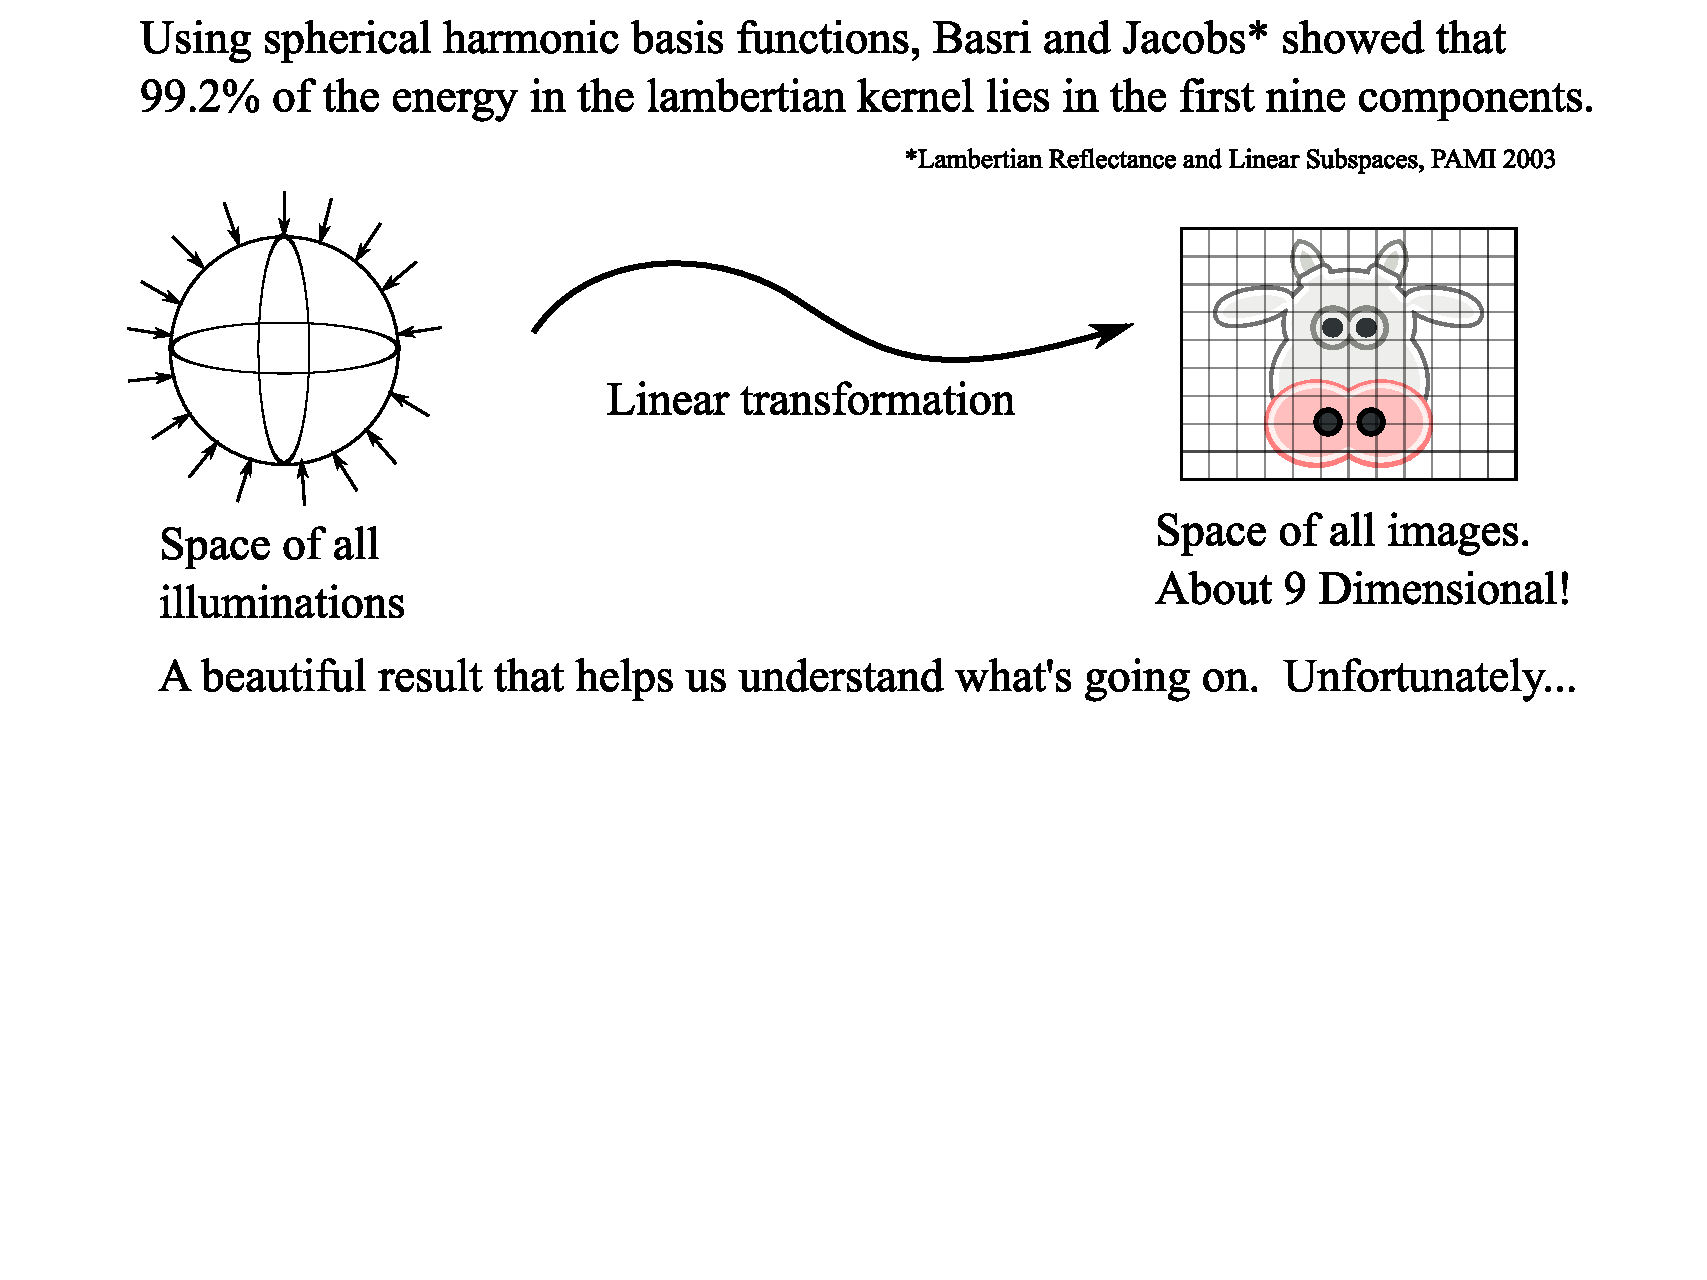
\includegraphics[width=0.8\textwidth]{images/basri3.pdf}
%\end{center}
%}

%\frame{
%\frametitle{Per-user alignment}
%\begin{center}
%%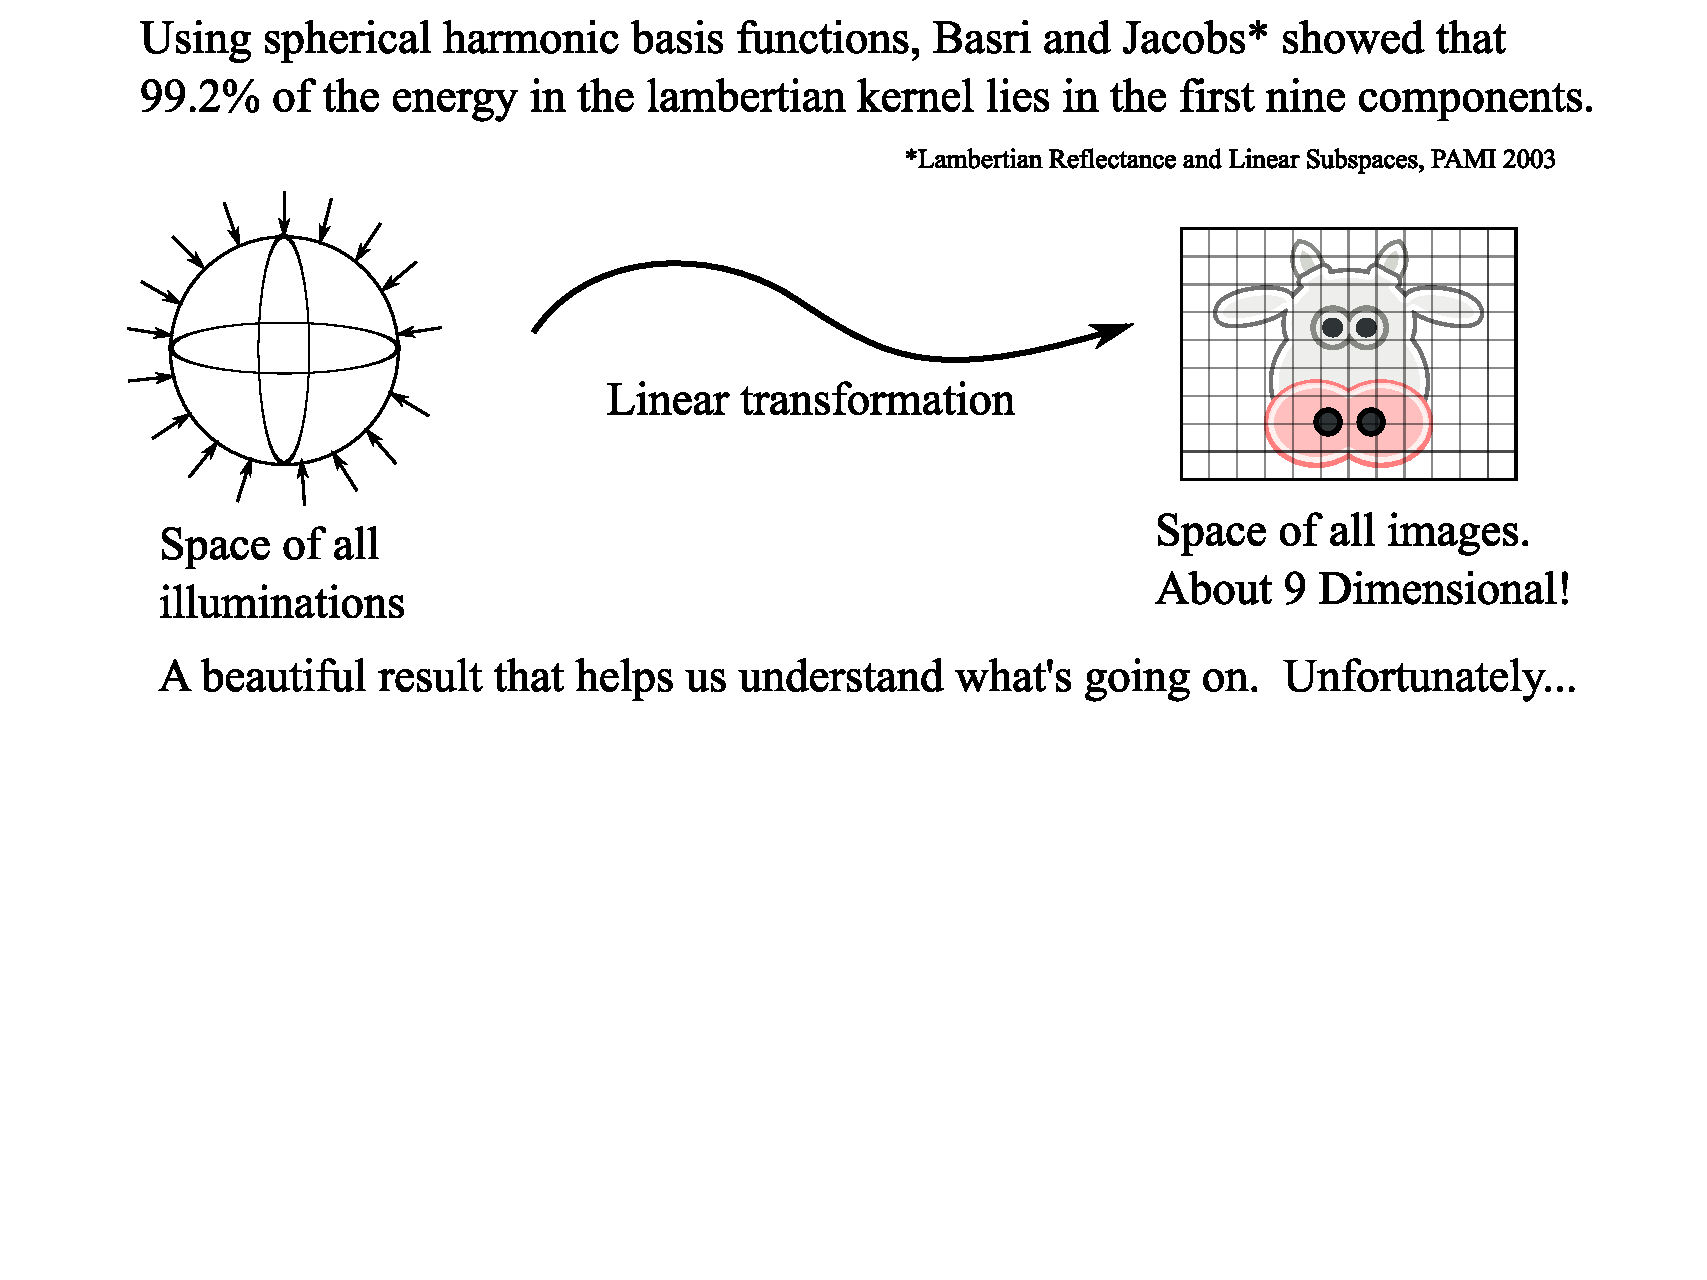
\includegraphics[width=0.8\textwidth]{images/basri3.pdf}
%\end{center}
%}

%\frame{
%\frametitle{Resampling the training images}
%\begin{center}
%%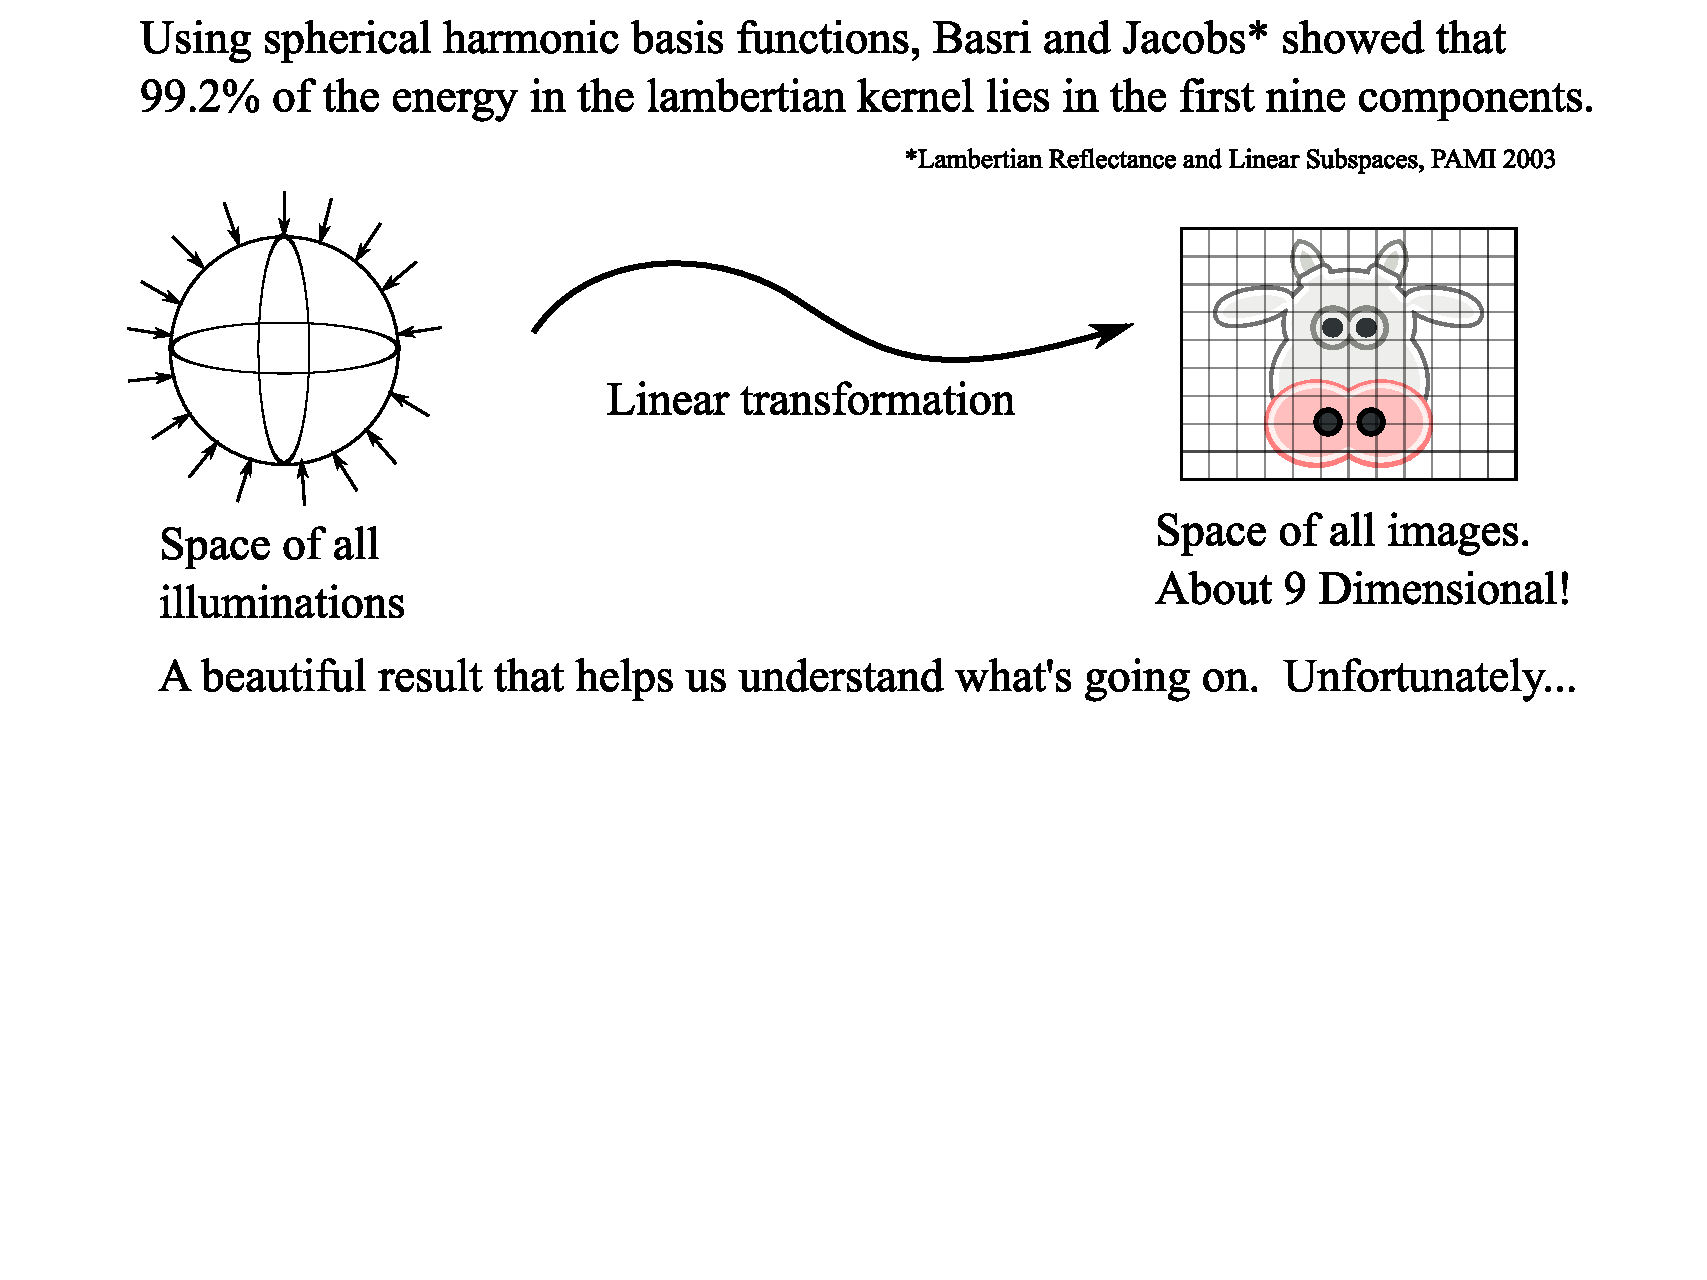
\includegraphics[width=0.8\textwidth]{images/basri3.pdf}
%\end{center}
%}

%\frame{
%\frametitle{Final recognition step}
%\begin{center}
%%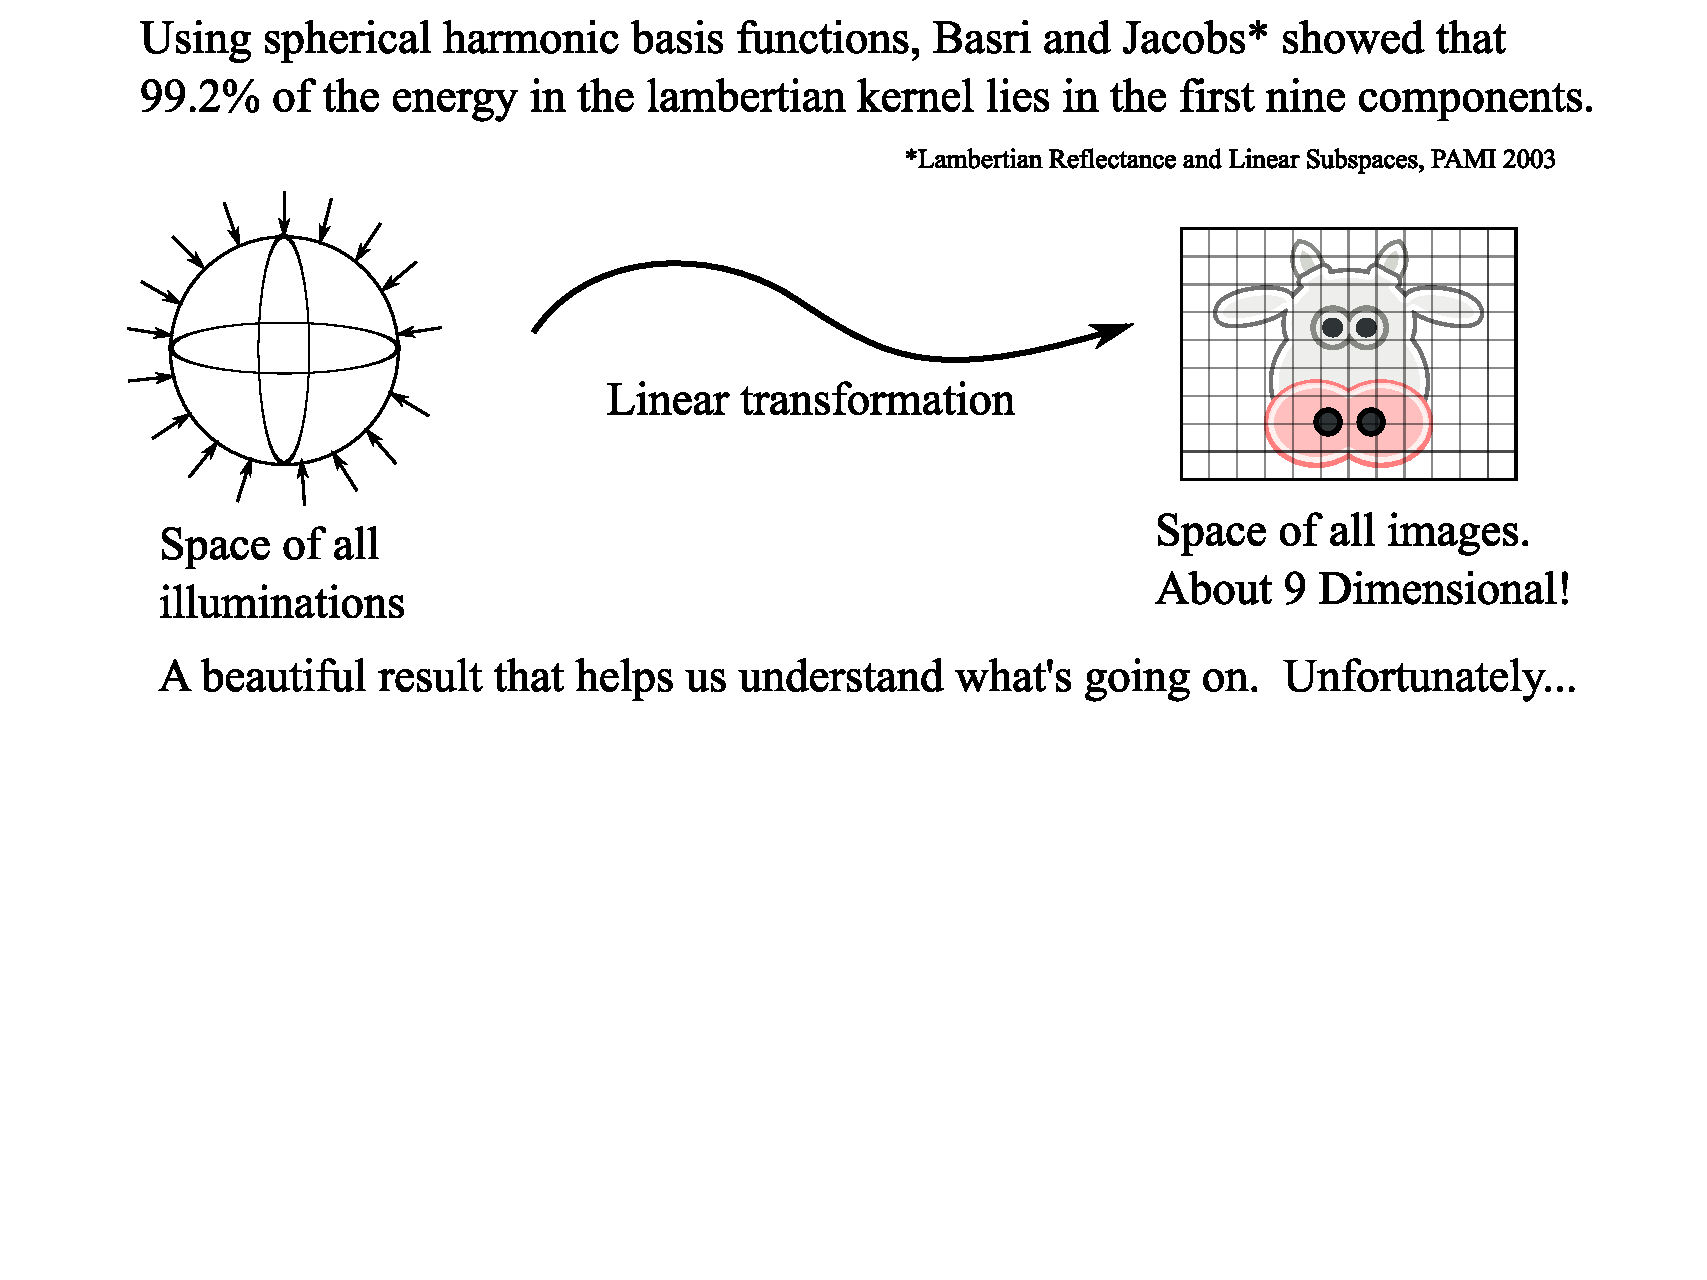
\includegraphics[width=0.8\textwidth]{images/basri3.pdf}
%\end{center}
%}

%\subsection{Optimizing the training illuminations}
%\frame{
%\frametitle{Optimize illuminations within the set of training images we already have}
%\begin{center}
%%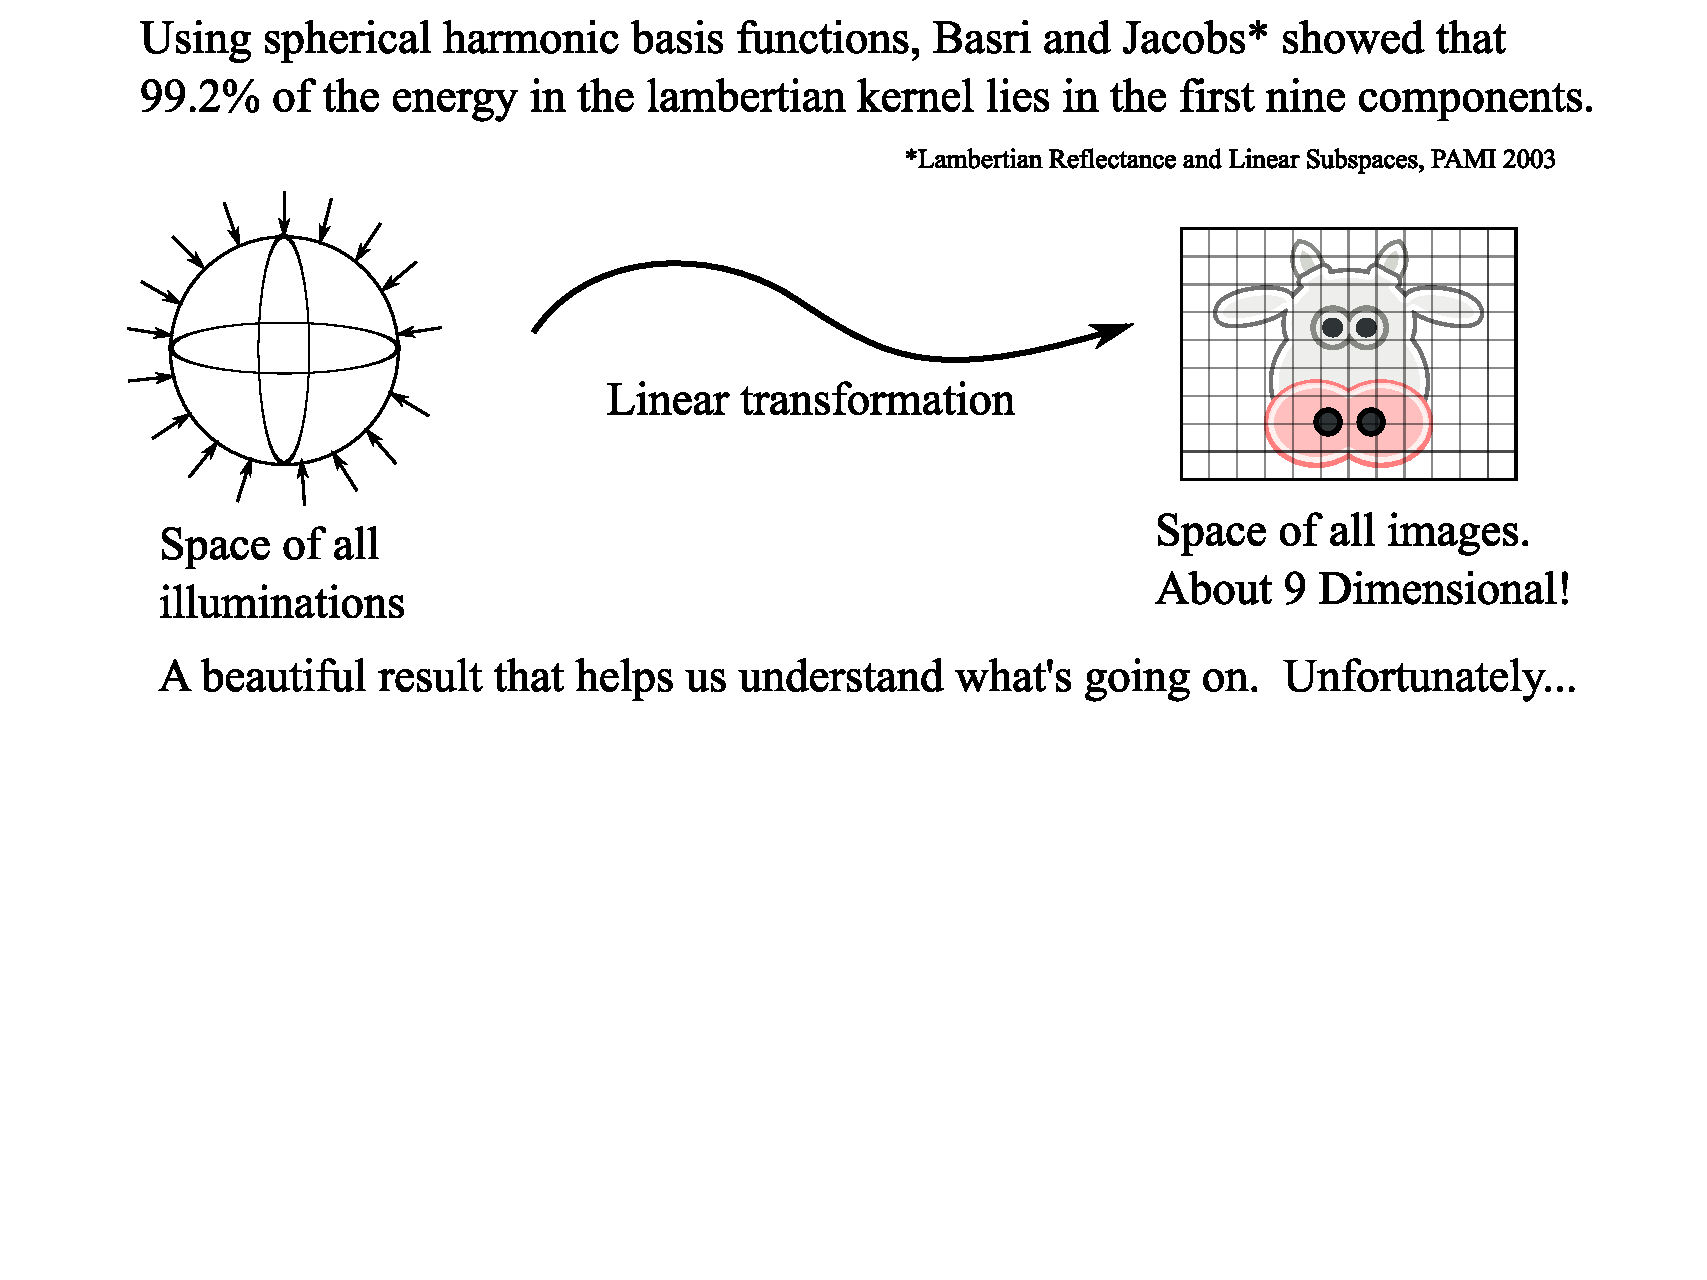
\includegraphics[width=0.8\textwidth]{images/basri3.pdf}
%\end{center}
%}

%\frame{
%\frametitle{Optimize illuminations with the illumination system in the loop}
%\begin{center}
%%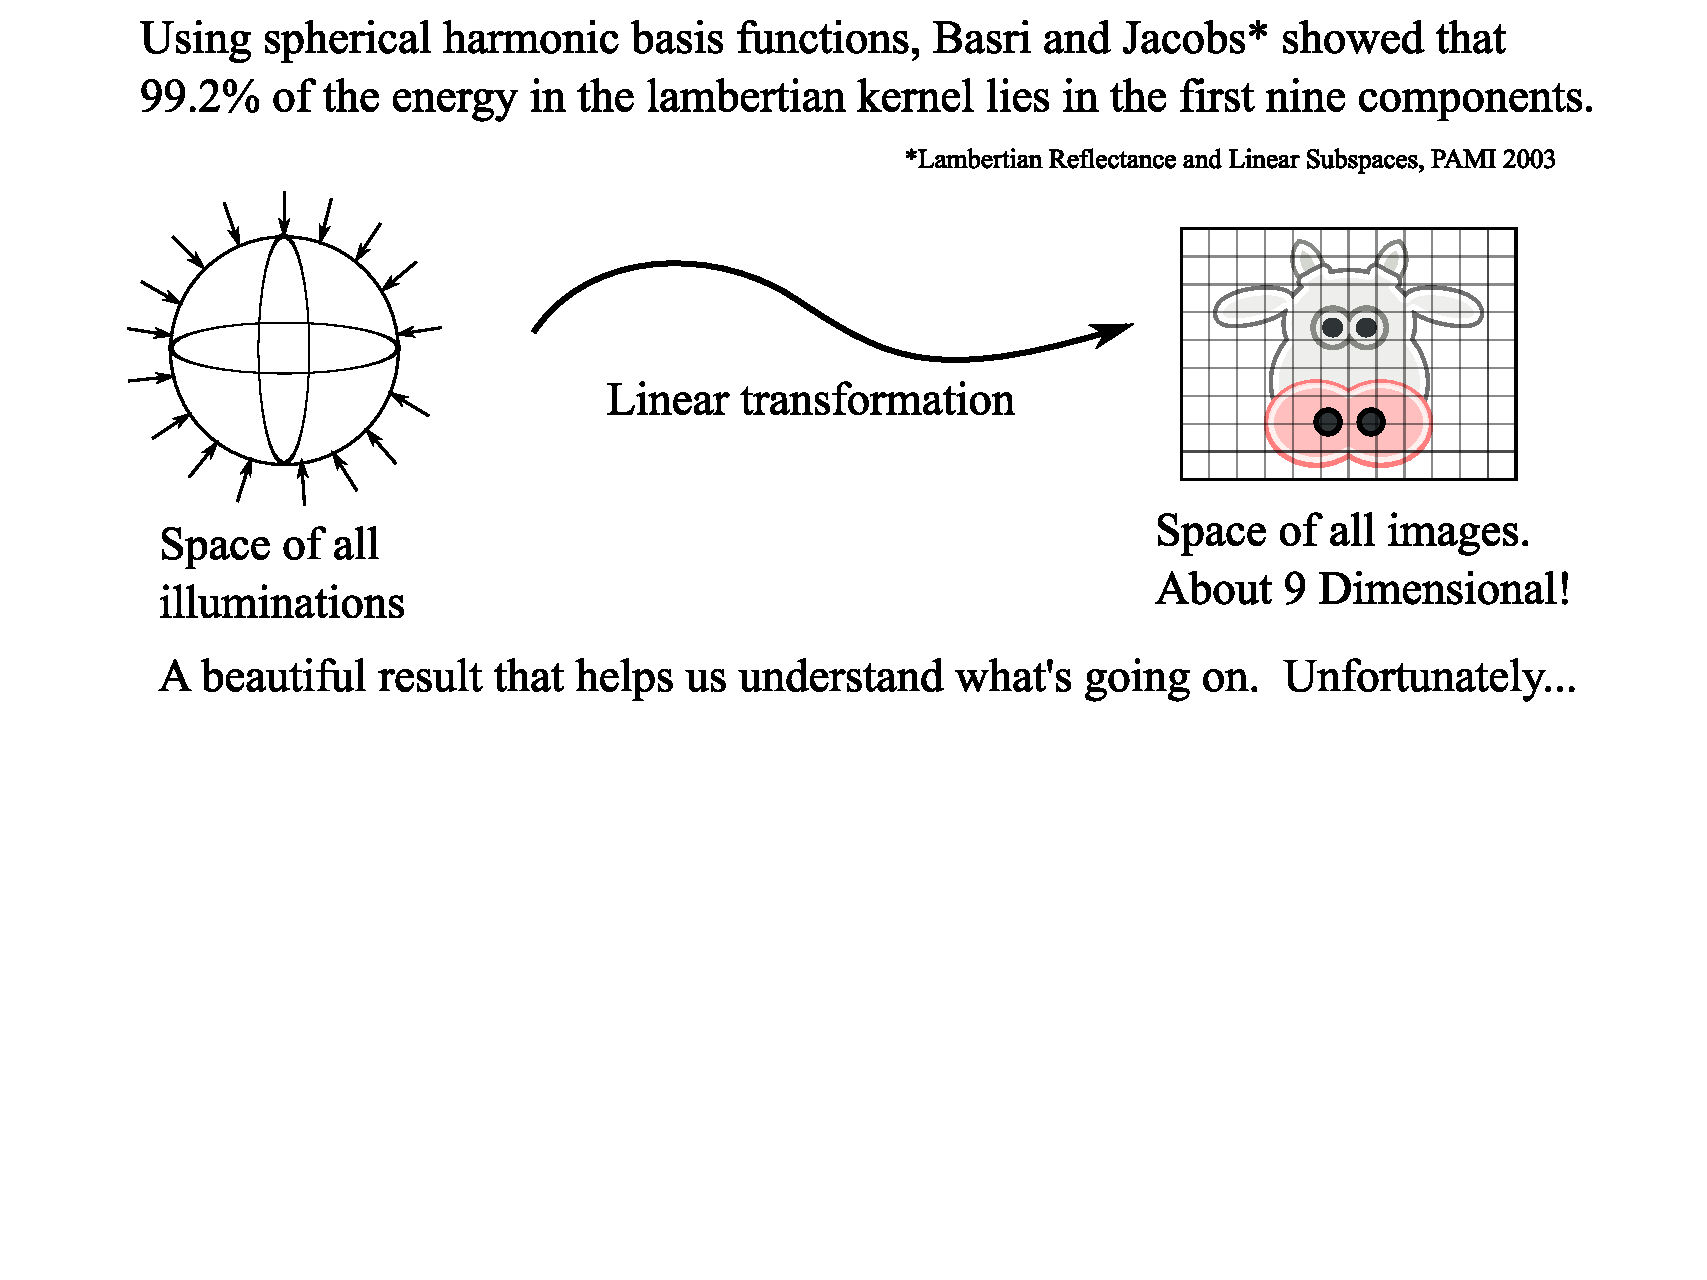
\includegraphics[width=0.8\textwidth]{images/basri3.pdf}
%\end{center}
%}

